\documentclass{beamer}

\usepackage{framed}
\usepackage{graphicx}

\begin{document}
\section{Plotting Bivariate Bistributions}
\begin{frame}[fragile]
\large
\noindent \textbf{Plotting Bivariate Bistributions}

	\begin{itemize}
\item It can also be useful to visualize a bivariate distribution of two variables. 
\item The easiest way to do this in seaborn is to just the \texttt{jointplot()} function, which creates a multi-panel figure that shows both the bivariate (or joint) relationship between two variables along with the univariate (or marginal) distribution of each on separate axes.
	\end{itemize}


\end{frame}
%==============================================================%

\begin{frame}[fragile]
	\frametitle{Seaborn Workshop}
	\large
\begin{framed}
\begin{verbatim}
mean, cov = [0, 1], [(1, .5), (.5, 1)]

data = np.random.multivariate_normal(mean, 
       cov, 200)

df = pd.DataFrame(data, columns=["x", "y"])
\end{verbatim}
\end{framed}

\end{frame}
%==============================================================%
\section{Scatterplots}
\begin{frame}[fragile]
	\large
	\begin{itemize}
\item The most familiar way to visualize a bivariate distribution is a scatterplot, where each observation is shown with point at the x and y values. 
\item This is analgous to a rug plot on two dimensions. 
\item You can draw a scatterplot with the matplotlib \texttt{plt.scatter} function, and it is also the default kind of plot shown by the \texttt{jointplot()} function:
	\end{itemize}


\end{frame}

%===========================================================%
\begin{frame}[fragile]
	\frametitle{Seaborn Workshop}
	\large
	\begin{framed}
\begin{verbatim}
sns.jointplot(x="x", y="y", data=df);
\end{verbatim}
\end{framed}
\begin{figure}
\centering
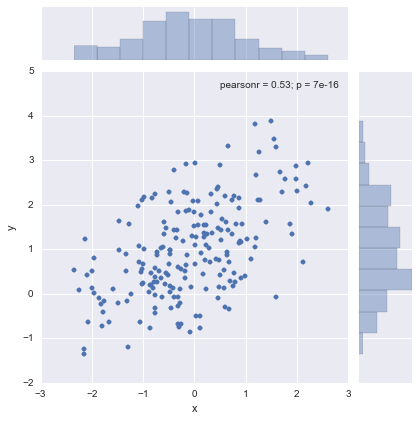
\includegraphics[width=0.55\linewidth]{images/distributions_30_0}
\end{figure}

\end{frame}
\section{Hexbin Plots}
%===========================================================%
\begin{frame}[fragile]
\noindent \textbf{Hexbin plots}
\begin{itemize}
\item The bivariate analogue of a histogram is known as a “hexbin” plot, because it shows the counts of observations that fall within hexagonal bins. \item This plot works best with relatively large datasets. 
\item It’s availible through the matplotlib \texttt{plt.hexbin} function and as a style in \texttt{jointplot()}. 
\item It looks best with a white background:
\end{itemize}

\end{frame}
%===========================================================%
\begin{frame}[fragile]
\begin{verbatim}
x, y = np.random.multivariate_normal(mean, cov, 1000).T
with sns.axes_style("white"):
sns.jointplot(x=x, y=y, kind="hex", color="k");
\end{verbatim}

\begin{figure}
\centering
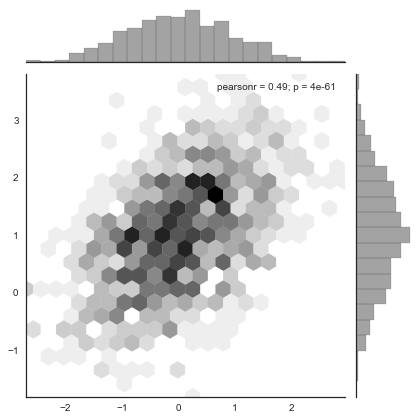
\includegraphics[width=0.7\linewidth]{images/distributions_32_0}

\end{figure}

\end{frame}
%===========================================================%
\begin{frame}[fragile]
\frametitle{Kernel density estimation}
\large
\begin{itemize}
\item It is also posible to use the kernel density estimation procedure described above to visualize a bivariate distribution. 
\item In seaborn, this kind of plot is shown with a contour plot and is available as a style in \texttt{jointplot()}:
\end{itemize}

\end{frame}
%===========================================================%
\begin{frame}[fragile]
\frametitle{Seaborn Workshop}
\large
	\begin{framed}
\begin{verbatim}
sns.jointplot(x="x", y="y", data=df, kind="kde");
\end{verbatim}
\end{framed}
\begin{figure}
\centering
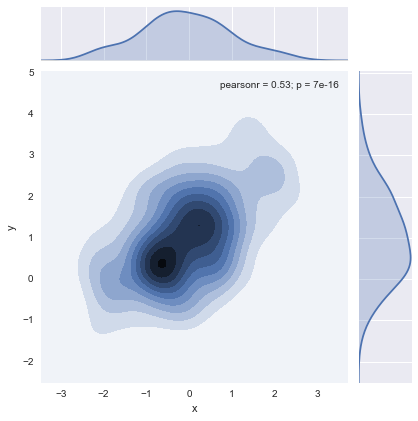
\includegraphics[width=0.55\linewidth]{images/distributions_34_0}
\end{figure}
\end{frame}
%===========================================================%
\begin{frame}[fragile]
\frametitle{Seaborn Workshop}
\large
	\begin{itemize}
\item You can also draw a two-dimensional kernel density plot with the \texttt{kdeplot()} function.
\item  This allows you to draw this kind of plot onto a specific (and possibly already existing) matplotlib axes, whereas the \texttt{jointplot()} function manages its own figure:
\end{itemize}
\end{frame}
%===========================================================%
\begin{frame}[fragile]
\begin{framed}
	\begin{verbatim}
f, ax = plt.subplots(figsize=(6, 6))
sns.kdeplot(df.x, df.y, ax=ax)
sns.rugplot(df.x, color="g", ax=ax)
sns.rugplot(df.y, vertical=True, ax=ax);
\end{verbatim}
\end{framed}
\begin{figure}
\centering
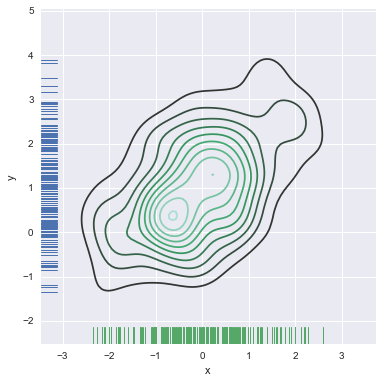
\includegraphics[width=0.55\linewidth]{images/distributions_36_0}
\end{figure}

\end{frame}
%===========================================================%
\begin{frame}[fragile]
	\large
If you wish to show the bivariate density more continuously, you can simply increase the number of contour levels:
\begin{verbatim}
f, ax = plt.subplots(figsize=(6, 6))
cmap = sns.cubehelix_palette(as_cmap=True, dark=0, light=1, reverse=True)
sns.kdeplot(df.x, df.y, cmap=cmap, n_levels=60, shade=True);
\end{verbatim}
\end{frame}
%===========================================================%
\begin{frame}[fragile]
\frametitle{Hexbin Plots}
	\large
\begin{figure}
\centering
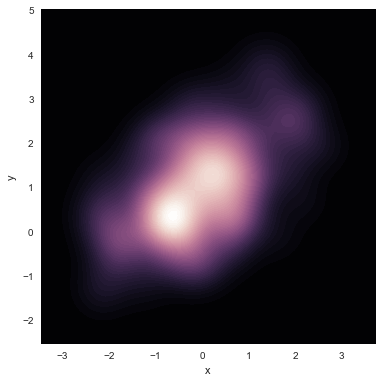
\includegraphics[width=0.55\linewidth]{images/distributions_38_0}
\end{figure}


\end{frame}
%===========================================================%
\begin{frame}[fragile]
\frametitle{Seaborn Workshop}
\large
	\begin{itemize}
\item The \texttt{jointplot()} function uses a \texttt{JointGrid} to manage the figure. \bigskip
\item For more flexibility, you may want to draw your figure by using \texttt{JointGrid} directly. \bigskip
\item  \texttt{jointplot()} returns the \texttt{JointGrid} object after plotting, which you can use to add more layers or to tweak other aspects of the visualization:
	\end{itemize}




\end{frame}
%===========================================================%
\begin{frame}[fragile]
\frametitle{Seaborn Workshop}	\large
	
\begin{framed}
\begin{verbatim}
g = sns.jointplot(x="x", y="y", 
    data=df, kind="kde", color="m")
    
g.plot_joint(plt.scatter, c="w", 
    s=30, linewidth=1, marker="+")
    
g.ax_joint.collections[0].set_alpha(0)

g.set_axis_labels("$X$", "$Y$");
\end{verbatim}
\end{framed}
\end{frame}
%===========================================================%
\begin{frame}[fragile]
	\large
	\begin{figure}
\centering
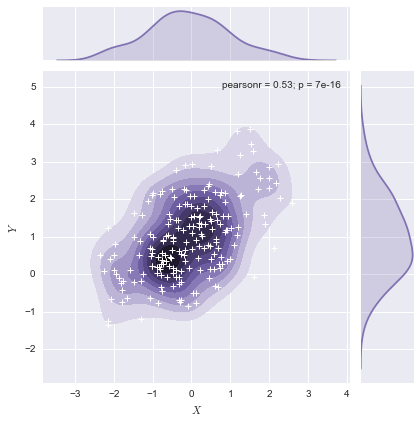
\includegraphics[width=0.55\linewidth]{images/distributions_40_0}
\end{figure}


\end{frame}

\end{document}